%%%%%%%%%%%%%%%%%%%%%%%%%%%%%%%%%%%%%%%%%%%%%%%%%%%%%%%%%%
%  Copyright (C) 2005 WanT group                         %
%  This file is distributed under the terms of the       %
%  GNU General Public License.                           %
%  See the file `License'  in the root directory of      %
%  the present distribution,                             %
%  or http://www.gnu.org/copyleft/gpl.txt                %
%%%%%%%%%%%%%%%%%%%%%%%%%%%%%%%%%%%%%%%%%%%%%%%%%%%%%%%%%%
\thispagestyle{empty}
\section{Theoretical Background}
\label{section:intro}

\noindent \WANT\ is an open-source, GNU General Public License
suite of codes that provides an integrated approach for the study
of coherent electronic transport in low-dimensional, extended
nanostructures. The core methodology combines state-of-the-art
Density Functional Theory (DFT), plane-waves, pseudopotential
calculations with a Green's functions method based on the Landauer
formalism to describe quantum conductance. The essential
connection between the two, and a crucial step in the calculation,
is the use of the maximally-localized Wannier function
representation to introduce naturally the ground-state electronic
structure into the lattice Green's function approach at the basis
of the evaluation of the quantum conductance. Moreover, the
knowledge of Wannier functions allows for a
direct link between the electronic transport properties of the
device with the nature of the chemical bonds, providing insight
into the mechanisms that govern electron flow at the nanoscale.
\\

\noindent \WANT\ scheme was originally described in Ref.~\cite{calz+04prb}:\\
A. Calzolari, N. Marzari, I. Souza, and M. Buongiorno Nardelli,\\
{\em Phys. Rev. B} {\bf 69}, 035108 (2004).
\\

\noindent In the following we review the theoretical background
that holds the \WANT\ method.


\subsection{Quantum transport}\label{subsec:tran}
%
Calculations of the quantum conductance are based on a
recently developed efficient method for evaluating quantum
transport in extended
systems~\cite{buon99prb,buon99prbr,buon+01prb}. This method is
applicable to any Hamiltonian that can be expanded within a
localized-orbital basis and can be used as a general theoretical
scheme for the computation and analysis of the electrical
properties of nanostructures.

\subsubsection{Electron transmission and Green's functions}
%
Let us consider a system composed of a conductor, $C$,
connected to two semi-infinite leads, $R$ and $L$, as in Fig.
\ref{fig:LCR}. A fundamental result in the theory of electronic
transport is that the zero-temperature conductance through a region of 
non-interacting
electrons (the $C$ region in Fig. \ref{fig:LCR}) is related to the
scattering properties of the region itself via the Landauer
formula~\cite{Landauer}:
%
%
\begin{equation}
{\mathcal C} = {2 e^2 \over h} {\mathcal T}(E_f),
\end{equation}
%
%
where ${\mathcal T}$ is the transmission function, ${\mathcal
C}$ is the conductance and $E_f$ the Fermi energy. 
The former represents the probability that
an electron injected at one end of the conductor will transmit to
the other end. In principle, we can compute the transmission
function for a coherent conductor\footnote{A conductor is said to
be coherent if it can be characterized by a transmission matrix
that relates each of the outgoing wave amplitudes to the incoming
wave amplitudes at a given energy.} starting from the knowledge of
the scattering matrix, $S$. The latter is the mathematical
quantity that describes the response at one lead due an excitation
at another. In principle, the scattering matrix can be uniquely
computed from the solution of the Schroedinger equation and would
suffice to describe the transport processes we are interested in
this work. However, it is a general result of conductance theory
that the elements of the S-matrix can be expressed in terms of the
Green's function of the conductor
\cite{datt95book,fish-lee81prb,meir-wing92prl} which, in practice,
can be sometimes simpler to compute.

Let us consider a physical system represented by an
Hamiltonian $H$. The Green's functions of the system can be
defined as: 
%
%
\begin{equation}
\label{eq:GF_def}
(\omega \pm i\eta-H) \, G(\omega)=I
\end{equation}
%
%
where $I$ is ht eidentity operator and 
$i\eta>0$ is an infinitesimal imaginary part added to the
energy to incorporate the boundary conditions into the equation.
The solution with $+$ sign is the retarded Green's function $G^r$,
while the solution with $-$ sign is called advanced Green's
function $G^a$. The transmission function can then be expressed in
terms of the Green's functions of the conductor and the couplings
of the conductor to the leads in a simple manner using the Fisher
and Lee formula~\cite{fish-lee81prb}:
%
%
\begin{equation}
{\mathcal T}(\omega) = {\rm Tr} \left[ 
            \Gamma_L G_C^r \Gamma_R G_C^a \right].
\label{eq:T}
\end{equation}
%
%
Here $G_C^{\{r,a\}}$ are the retarded and advanced
Green's functions of the conductor, and $\Gamma_{\{L,R\}}$ are
functions that describe the coupling of the conductor to the leads.

In the following we are going to restrict the discussion
to discrete systems that we can describe by ordinary matrix
algebra. More precisely, we are going to work with matrices
representing a physical system in the basis of localized
electronic orbitals centered on the atoms constituting the system.
It includes in particular the tight-binding model.
For a discrete media, the Green's function defined in Eq.~(\ref{eq:GF_def}) 
is then the inverse of the $(\omega - H)$ matrix.
To simplify the notation, we drop
the exponentis $\{a,r\}$ referring to advanced and retarded
functions and include the $\pm i\eta$ factor in $\omega$. For an open
system, consisting of a conductor and two semi-infinite leads (see
Fig. \ref{fig:LCR}), the above Green's function can be partitioned
into sub-matrices that correspond to the individual subsystems:
%
%
\begin{equation}
\left(
\begin{array}{lll}
g_L� & g_{LC} &� g_{LCR}\\
g_{CL} & G_C & g_{CR} \\
g_{LRC} & g_{RC} & g_R
\end{array}
\right) = \left(
\begin{array}{ccc}
\omega -h_L & -h_{LC} & 0\\
-h_{LC}^\dagger & \omega -H_C & -h_{CR}\\
0 & -h_{CR}^\dagger & \omega -h_R
\end{array}
\right)^{-1}, \label{condmatr}
\end{equation}
%
%
where the matrix $(\omega -H_C)$ represents the finite
``isolated'' conductor (with no coupling elements to the leads),
$(\omega -h_{\{R,L\}})$ represent the semi-infinite leads, and
$h_{CR}$ and $h_{LC}$ are the coupling matrices between the
conductor and the leads.
As a convention, we use lower case
letters for (semi-)infinite matrices and upper case for finite
dimension matrices. In Eq.~(\ref{condmatr}) we have made the
assumption that there is no direct interaction between the left
and right leads. From this equation it is straightforward to
obtain an explicit expression for $G_C$\cite{datt95book}:
%
%
\begin{equation}
   G_C(\omega) = (\omega -H_C -\Sigma_L(\omega) -\Sigma_R(\omega))^{-1} 
   \label{gconduct}
\end{equation}
%
%
where the finite dimension matrices
%
%
\begin{equation}
  \Sigma_L(\omega) = h_{LC}^\dagger (\omega -h_L)^{-1} h_{LC}, \;\;\;\;
  \Sigma_R(\omega) = h_{RC} (\omega -h_R)^{-1} h_{RC}^\dagger
\end{equation}
%
%
are defined as the self-energies due to the
semi-infinite leads. These terms can be viewed as
effective Hamiltonians that arise from the coupling of the
conductor with the leads. The coupling functions
$\Gamma_{\{L,R\}}(\omega)$ can then be obtained as~\cite{datt95book}:
%
%
\begin{equation}
   \Gamma_{\{L,R\}} = {\rm i} \left[ \Sigma_{\{L,R\}}^r(\omega) -
                      \Sigma_{\{L,R\}}^a(\omega) \right], 
   \label{eq:gamma}
\end{equation}
%
%
where the advanced self-energy $\Sigma_{\{L,R\}}^a$ is
the Hermitian conjugate of the retarded self-energy
$\Sigma_{\{L,R\}}^r$. The core of the problem lies in the
calculation of the self-energies of the semi-infinite leads.
%
%
\begin{figure}
   \begin{center}
     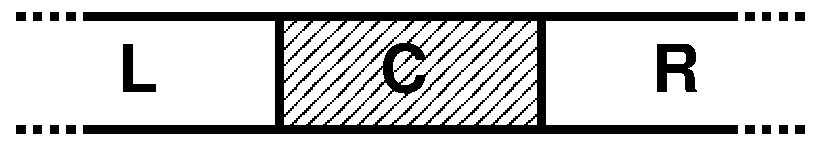
\includegraphics[width=0.45\textwidth]{fig1}
     \caption{A conductor described by the Hamiltonian $H_C$, connected
              to two semi-infinite leads $L$ and $R$, through the coupling
              matrices $h_{LC}$ and $h_{CR}$. \label{fig:LCR} }
   \end{center}
\end{figure}

It is well known that any solid (or surface) can be
viewed as an infinite (semi-infinite in the case of surfaces)
stack of principal layers with nearest-neighbor interactions
\cite{lee-joan81prb,lee-joan81prb1}. This corresponds to
transforming the original system into a linear chain of principal
layers. For a lead-conductor-lead system, the conductor can be
considered as one principal layer sandwiched between two
semi-infinite stacks of principal layers. The next sections
are devoted to the computation of the self-energies using the
principal layers approach.

%%%%%%%%%%%%%%%%%%%%%%%%%%%%%%%%%%%%%%%%%%%%%%%%%%%%%%%%%%%%%%%%%%%

\subsubsection{Transmission through a bulk system.} 
\label{ss:bulk}
%
Within the principal layer approach, the matrix elements
of Eq.~(\ref{eq:GF_def}) between layer orbitals yield a series of
matrix equations for the Green's functions:
%
%
\begin{eqnarray}
\label{serie}
    (\omega -H_{00}) G_{00} & = & I + H_{01}G_{10}\\
\nonumber
    (\omega -H_{00}) G_{10} & = & H_{01}^\dagger G_{00} + H_{01}G_{20}\\
\nonumber
                        \dots\\
\nonumber
    (\omega -H_{00}) G_{n0} & = & H_{01}^\dagger G_{n-1,0} +
                        H_{01}G_{n+1,0}
\end{eqnarray}
%
%
where the finite dimension matrices $H_{nm}$ and
$G_{nm}$ are formed by the matrix elements of the Hamiltonian and
Green's function between the layer orbitals. We assume that in a
bulk system $H_{00}=H_{11}=\dots$ and $H_{01}=H_{12}=\dots$.
Following Refs.~\cite{LopezSancho1,LopezSancho2}, this chain can be
transformed in order to express the Green's function of an
individual layer in terms of the Green's function of the preceding
(or following) one. This is done via the introduction of the
transfer matrices $T$ and $\overline{T}$, defined such that
$G_{10}=TG_{00}$
and $G_{00}=\overline{T}G_{10}$.
Using these definitions, we can write the bulk Green's
function as~\cite{Garcia2}:
%
%
\begin{equation}
    \label{eq:GT} G(\omega) = (\omega - H_{00} - H_{01}T
                  -H_{01}^\dagger \overline{T})^{-1}.
\end{equation}
%
%
The transfer matrix can be easily computed from the
Hamiltonian matrix elements via an iterative procedure, as
outlined in \cite{LopezSancho1,LopezSancho2}. In particular $T$
and $\overline T$ can be written as:
%
%
\begin{eqnarray}
   T &=& t_0 + \tilde{t}_0t_1 + \tilde{t}_0\tilde{t}_1t_2+\ldots+
   \tilde{t}_0\tilde{t}_1\tilde{t}_2\cdots t_n  \, ,\\
\nonumber
   \overline T &=& \tilde{t}_0 + t_0\tilde{t}_1 +t_0t_1\tilde{t}_2
   +\ldots+ t_0t_1t_2\cdots\tilde{t}_n \, ,
\end{eqnarray}
%
%
where $t_i$ and $\tilde{t}_i$ are defined via the recursion
formulas:
%
%
\begin{eqnarray}
   t_i &=& (I -t_{i-1}\tilde{t}_{i-1} - \tilde{t}_{i-1}t_{i-1})^{-1}
   t_{i-1}^2 , \\
   \tilde{t}_i &=& (I -t_{i-1}\tilde{t}_{i-1} -
   \tilde{t}_{i-1}t_{i-1})^{-1} \tilde{t}_{i-1}^2 ,
\nonumber
\end{eqnarray}
%
%
and
%
%
\begin{eqnarray}
   t_0 &=& (\omega - H_{00})^{-1} H_{01}^\dagger,\\
   \tilde{t}_0 &=& (\omega - H_{00})^{-1} H_{01}.
\nonumber
\end{eqnarray}
%
%
\noindent The process is repeated until $t_n,\tilde{t}_n \le
\delta$ with $\delta$ arbitrarily small. Usually, no more than 5 or
6 iterations are required to converge the above sum.

If we compare Eq.~(\ref{eq:GT}) with Eq.~(\ref{gconduct}), 
in the hypothesis of leads and conductors being
of the same material (bulk conductivity), we can identify one
principal layer of the bulk system with the conductor $C$, so that
$H_{00}\equiv H_C$. In particular, by comparing with
Eq.(\ref{gconduct}), we obtain the expression of the self-energies
of the conductor-leads system:
%
%
\begin{equation}
\Sigma_L = H_{01}^\dagger \overline T, \;\;\;\;\; \Sigma_R = H_{01} T.
\label{eq:sigmabulk}
\end{equation}
%
%
The coupling functions are then obtained~\cite{buon99prb} from the sole
knowledge of the transfer matrices and the coupling Hamiltonian
matrix elements: $\Gamma_L=-{\rm Im}(H_{01}^\dagger \overline T)$ and
$\Gamma_R=-{\rm Im}(H_{01} \overline T)$.

%%%%%%%%%%%%%%%%%%%%%%%%%%%%%%%%%%%%%%%%%%%%%%%%%%%%%%%%%%%%%%%%%%%%

\subsubsection{Transmission through a left lead-conductor-right lead
(LCR) system.} \label{ss:LCR}
%
The procedure outlined above can also be applied to the
case of electron transmission through one or more interfaces,
between different media. For the calculation of conductances in
realistic experimental geometry, the method can be expanded to the
general configuration of a Left-lead-Conductor-Right-lead (LCR)
systems --- as displayed in Fig~.\ref{fig:LCR}. To study this case
we make use of the Surface Green's Function Matching (SGFM)
theory, pioneered by~\cite{Garcia1,Garcia2}.

We have to compute the Green's function $G_I$, where the
subscript $I$ refers to the interface region composed of two
principal layers --- one in each media --- (L, C, R in our case).
Using the SGFM method, $G_I$ is calculated from the bulk Green's
function of the isolated systems,  and the coupling between the
two principal layers at the two sides of the interface. Via the
calculation of the transmitted and reflected amplitudes of an
elementary excitation that propagates from one medium to another,
it can be shown that the interface Green's function obeys the
following secular equation~\cite{Garcia2}:
%
%
\begin{eqnarray}
\nonumber G_{LCR}&=& \left(
\begin{array}{ccc}
G_{L} & G_{LC} & G_{LR}\\
G_{CL} & G_{C} & G_{CR}\\
G_{RL} & G_{RC} & G_{R}\\
\end{array}
\right) \\ &=& \left(
\begin{array}{ccc}
\omega -H^L_{00} - H^L_{01 \, \dagger} \overline T & -H_{LC} & 0\\
-H_{CL} & \omega -H_{C} & -H_{CR}\\
0 & -H_{RC} & \omega -H^R_{00} - H^R_{01} T \\
\end{array}
\right)^{-1}. \label{secular1}
\end{eqnarray}
%
%
where $H_{nm}^{\{L,R\}}$ are the block matrices of the
Hamiltonian between the layer orbitals in the left and right leads
respectively, and $T_{\{L,R\}}$ and $\overline{T}_{\{L,R\}}$ are
the appropriate transfer matrices. The latter are easily computed
from the Hamiltonian matrix elements via the iterative procedure
already described in the bulk case (Sec.\ref{ss:bulk}).
Correspondingly, $H_{LC}$ and $H_{CR}$ are the coupling matrices
between the conductor and the leads principal layers in contact
with the conductor.
It is straightforward to obtain in the form of
Eq.(\ref{gconduct}), $G_C = (\omega -H_C -\Sigma_L
-\Sigma_R)^{-1}$, where $\Sigma_{L}$ and $\Sigma_R$ are the
self-energy terms due to the semi-infinite leads, and
identify~\cite{buon99prb}:
%
%
\begin{equation}
  \begin{array}{ccl}
  \Sigma_L(\omega) & = & H_{LC}^{\dagger} \, \Big(
                   \omega -H_{00}^L \,-H_{01}^{L\, \dagger}
                   \, \overline T_L \Big)^{-1} \, H_{LC},\\ 
  \Sigma_R(\omega) & = & H_{CR} \, \Big(\omega
                  -H_{00}^R-H_{01}^R \,T_R \Big)^{-1} \, H_{CR}^\dagger.
  \end{array}
\end{equation}
%
%
The transmission function in the LCR geometry can then
be derived from Eq.(\ref{eq:T}) and (\ref{eq:gamma}).
%
The knowledge of the conductor's Green's function $G_C$
gives also direct information on the electronic spectrum of the
system via the spectral density of states:
%
%
\begin{equation}
   N(\omega)= -\frac{1}{\pi} {\rm Im}\, {\rm Tr} \, G_C(\omega) .
\end{equation}
%
%
We have assumed a truly one-dimensional chain of
principal layers, which is physical only for systems like
nanotubes or quantum wires that have a definite
quasi-one-dimensional character. The extension to a truly
three-dimensional case is straightforward using Bloch functions in
the directions perpendicular to the transport axis. The introduction
of the principal layer concept implies that along the direction of
the layer expansion the system is described by an infinite set of
$k_\bot$ while $k_\|$ are still good quantum numbers for the
problem. The above procedure effectively reduces the
three-dimensional system to a set of non-interacting
linear-chains, one for each $k_\|$~\cite{lee-joan81prb,lee-joan81prb1}. 
We can then use the usual $k$-point summation techniques to evaluate the
quantum conductance: 
%
%
\begin{equation}
    T(\omega) = \sum_{k_\|} w_{k_\|}T_{k_\|}(\omega)
\end{equation}
%
%
where $w_{k_\|}$ are the relative weights of the different $k_\|$
in the irreducible wedge of the surface Brillouin 
zone~\cite{Baldereschi:1}.

%%%%%%%%%%%%%%%%%%%%%%%%%%%%%%%%%%%%%%%%%%%%%%%%%%%%%%%%%%%%%%%%%%%


\subsection {Maximally localized Wannier functions}\label{subsec:wannier}
%
\subsubsection{Definition of the problem}
%
Bloch orbitals cannot be used directly to evaluate
electronic transport with the method outlined in Sec.~\ref{subsec:tran}. 
As we have pointed out, quantum conductance
is computed starting from the knowledge of the lattice Green's
function, whose calculation relies on a localized orbital
representation. Bloch
orbitals, that are intrinsically delocalized, have to be
transformed into {\em localized} functions in order to construct
the sparse, short-ranged matrix elements of the Hamiltonian. The
core of our proposed methodology is to use m{\em
aximally-localized Wannier functions} (WFs) for the system
considered. These are the most natural choice for a set of
localized orbitals that still span the same Hilbert space of the
Hamiltonian eigenfunctions: they allow to bridge plane-wave
electronic structure and lattice Green's function calculations in
a coherent fashion.

A Wannier function $w_{n{\bf R}}({\bf r})$, labeled by
the Bravais lattice vector {\bf R}, is usually defined via a
unitary transformation of the Bloch functions $\psi_{n{\bf
k}}({\bf r})$ of the $n$th band:
%
%
\begin{equation}
w_{n{\bf R}}({\bf r})=\frac{V}{(2\pi)^3}\int_{BZ}\psi_{n{\bf k}}({\bf r})
e^{-i{\bf k}\cdot{\bf R}} d^3k,
\label{wf}
\end{equation}
%
%
where V is the volume of the unit cell and the
integration is performed over the entire Brillouin Zone. It is
easy to show that the WFs defined as above form an orthonormal
basis set, and that any two of them, for a given index $n$ and
different ${\bf R}$ and ${\bf R^\prime}$, are just translational
images of each other. Note that, as WFs are
(continuous) linear combinations of Bloch functions with different
energies, they do not represent stationary states, but still span
the original Hilbert space.

The {\em ab-initio} eigenstates are well-defined,
modulus an arbitrary ${\bf k}$-dependent phase factor; thus, the
definition above does not lead to a unique set of Wannier
functions~\cite{kohn,kohn1}, since the electronic structure
problem is invariant for the transformation $\psi_{n{\bf k}}
\rightarrow e^{\phi_n({\bf k})} \psi_{n{\bf k}} $. Besides this
freedom in the choice of phases $\phi_n({\bf k})$ for the Bloch
functions, there is a more comprehensive gauge freedom stemming
from the fact that the many-body wavefunction is actually a Slater
determinant: a unitary transformation between orbitals will not
change the manifold, and will not change the total energy and the
charge density of the system. In all generality, starting with a
set of ${\mathcal N}$ Bloch functions with periodic parts
$u_{n{\bf k}}$, we can constructs infinite sets of ${\mathcal N}$
WFs displaying different spatial characteristics:
%
%
\begin{equation}
    w_{n{\bf R}}({\bf r})=\frac{V}{(2\pi)^3}\int_{BZ}
    \left[ \sum_m U_{mn}^{({\bf k})}
    \psi_{m{\bf k}}({\bf r}) \right]
    e^{-i{\bf k}\cdot{\bf R}} d^3k.
    \label{eq:MLWF}
\end{equation}
%
%
The unitary matrices $U^{({\bf k})}$ include also the
gauge freedom on phase factors afore mentioned~\cite{nicola}. \\

\noindent The present \WANT\ method is based on a localization algorithm
that allows to transform a set of Bloch functions -- calculated by means
of {\it ab initio} approaches -- into a unique set of Maximally localized
Wannier functions, as proposed by Marzari and Vanderbilt
in 1997~\cite{nicola}. The formulation of this minimum-spread
criterion extends the concept of \emph{localized molecular
orbitals}, proposed by Boys~\cite{boys} for molecules, to the
solid-state case. However, its generality allows to deal with both
``extended'' (periodic and disordered) systems as well as with
``isolated'' clusters and molecules, in the limit of large
supercells.

\subsubsection{Localization procedure}
%
For our purposes, we need to transform the Bloch
eigenstates in WFs with the narrowest spatial
distribution. Following the procedure proposed by Marzari and
Vanderbilt~\cite{nicola}, we search the particular unitary
matrix $U_{mn}^{({\bf k})}$ that transform the Bloch eigenstates
in the WFs with the narrowest spatial distribution.

A measure of the spatial delocalization of WFs is given
by a {\em Spread Operator} $\Omega$, defined as the sum of the
second moments of all the Wannier functions in a reference cell:
%
%
\begin{equation}
    \Omega=\sum_n [\langle r^2 \rangle_n - \langle {\bf r}
    \rangle_n^2] , \label{omega}
\end{equation}
%
%
where the sum is over a selected  group of bands, and
%
%
\begin{eqnarray}
    \langle {\bf r} \rangle_n &=&\langle {\bf 0}n | {\bf r} | {\bf 0}n \rangle, \\
    \nonumber
    \langle r^2 \rangle_n &=& \langle {\bf 0}n | r^2 | {\bf 0}n \rangle .
    \label{position}
\end{eqnarray}
%
%
The value of the spread $\Omega$ depends on the choice
of unitary matrices $U^{({\bf k})}$; thus  it is possible to
evolve any arbitrary set of $U^{({\bf k})}$ until we reach the stationarity
condition:
%
%
\begin{equation}
   \frac {\delta \Omega_{\bf k}}{\delta U^{({\bf k})}}=0
   \label{minimo}
\end{equation}
%
%
At the minimum, we obtain the matrices
$U^{({\bf k}), ML}$ that transform the first-principles
$\psi_{n{\bf k}}^{FP}({\bf r})$ into the {\em maximally-localized
WFs}, according to Eq.~(\ref{eq:MLWF}).
If we restrict to the case of {\bf k}-point mesh
calculations, we can use finite differences in reciprocal space to
evaluate the derivatives of Eq.~(\ref{minimo}). For this purpose we
rewrite the expectation values $\langle \mathbf{r} \rangle$ and 
$\langle r^2 \rangle $ as proposed by Blount~\cite{blount}:
%
%
\begin{eqnarray}
\label{eq:pos_k}
\langle {\bf 0}n | {\bf r} | {\bf 0}n  \rangle &=& i \frac{1}{N}
\sum_{ {\bf k} } e^{ +i{\bf k}\cdot{\bf R} } \langle u_{ {\bf k}n
}| \nabla_{\bf k} | u_{ {\bf k}n },  \rangle\\
%
\nonumber
\langle {\bf 0}n | r^2 | {\bf 0}n \rangle\ &=& \frac{1}{N} \sum_{
{\bf k}} e^{+i{\bf k}\cdot{\bf R}} \langle u_{ {\bf k}n }|
\nabla^2_{\bf k} | u_{ {\bf k}n }  \rangle, 
\end{eqnarray}
%
%
where $| u_{ n{\bf k} }  \rangle = e^{-i{\bf k}\cdot{\bf
r}} | \psi_{ n{\bf k} }  \rangle$ is the periodic part of the Bloch
function. Making the assumption that the BZ has been discretized
into a uniform {\bf k}-point mesh, and letting $ \mathbf{b} $ being 
the vectors
that connect a mesh point to its near neighbors, we can define the
overlap matrix between Bloch orbitals as:
%
%
\begin{equation}
   \label{overlap}
   M^{ ( \mathbf{k},\mathbf{b}) }_{ mn } = \langle u_{ m\mathbf{k} }| 
        u_{ n\mathbf{k}+\mathbf{b} }  \rangle = 
        \langle \psi_{ m \mathbf{k} } | e^{-i\mathbf{k}\mathbf{b}} | 
        \psi_{ n \mathbf{k}+\mathbf{b}} \rangle .
\end{equation}
%
%
Using the expression of the gradient  in terms of finite
differences and substituting $M^{ ({\bf k}, {\bf b})}_{ mn }$ in
Eq.~(\ref{eq:pos_k}) we obtain the expressions for $\langle \mathbf{r} \rangle$
and $\langle r^2 \rangle $
to be used in the localization procedure:
%
%
\begin{eqnarray}
\label{position2}
   \langle \mathbf{r} \rangle_{n} &=& -\frac{1}{N}
          \sum_{ \mathbf{k},\mathbf{b} } 
           w_b \, \mathbf{b} \, \text{Im} 
          \, \text{Ln} M^{ ({\bf k}, {\bf b})}_{ nn } \\ \nonumber
   \langle r^2 \rangle_n &=&  \frac{1}{N} \sum_{ {\bf k,b} } w_b
   \left[ \left( 1- |M^{ ({\bf k}, {\bf b}}_{ nn }|^2 \right) +
          \left( \text{Im}\, \text{Ln} M^{ ({\bf k}, {\bf b})}_{ nn } \right)^2 
   \right]
\end{eqnarray}
%
%
Here, $w_b$ are the weights of the $\mathbf{b}$-vectors, and
must satisfy the completeness condition $\sum_{\mathbf{b}} w_b
b_{\alpha}b_{\beta}= \delta_{{\alpha}{\beta}}$. Substituting the
above expression into Eq.~(\ref{omega}), we obtain the expression
for the spread operator as a function of the overlap matrix $M^{
({\bf k}, {\bf b})}_{ mn }$.

In order to calculate the gradient in Eq.~(\ref{minimo}),
we consider the first order change in $\Omega$ arising from an
infinitesimal transformation $U_{mn}^{({\bf k})} = \delta_{mn} +
dW_{mn}^{({\bf k})}$, where $dW$ is an infinitesimal antiunitary
matrix ($dW^{\dag} = - dW$). The gauge transformation rotates the
wave functions according to Eq.~(\ref{eq:MLWF}) into $| u_{ {\bf k}n }
\rangle \to | u_{ {\bf k}n } \rangle + \sum_mdW_{mn}^{({\bf k})}|
u_{ {\bf k}m } \rangle $. Following the elegant description of
Ref. \cite{nicola}, we obtain the final expression for the
gradient of the spread functional:
%
%
\begin{equation}
   \label{grad_fin}
   G^{({\bf k})}=\frac{\delta \Omega}{dW^{({\bf k})}}= 4 \sum_{ {\bf
   b} } w_b \left( \frac {R^{{\bf k,b})} -R^{({\bf
   k,b}) \, \dagger}}{2} - \frac {T^{({\bf k,b})}+T^{({\bf
   k,b}) \, \dagger}}{2i} \right)  
\end{equation}
%
%
where
%
%
\begin{equation}
   R_{mn}^{ ({\bf k,b}) } = M_{mn}^{ ({\bf k,b}) } M_{nn}^{ ({\bf
   k,b})\ast} ;\qquad T_{mn}^{ ({\bf k,b}) }= \frac{ M_{mn}^{ ({\bf
   k,b}) } } { M_{nn}^{ ({\bf k,b}) } } \left[ \text{Im}\, \text{Ln} M_{nn}^{({\bf
   k,b})} + {\bf b}\cdot \langle {\bf r} \rangle_n \right].
\end{equation}
%
%
Note that the entire expression $G^{({\bf k})}$ is a
function of the overlap matrices $M^{ ({\bf k,b}) }$.  The
minimization of the spread functional $\Omega$ is obtained via
steepest descent or conjugate gradient schemes.
The procedure does not require the updating of wavefunctions, but only
of the overlap and unitary matrixes. This is the most demanding task 
(scaling as $N^3$) for each iteration in Wannier localization.

Wannier functions obtained with the above procedure
should be almost real, except for an overall phase factor. 
This conjecture can also be used as a check of the convergence of the
localization procedure.
It is important to
notice that whenever a Born-von Karman discretization of the
Brillouin Zone is introduced, even the above-mentioned WFs are not
truly localized, but will be periodic in real-space, with a {\em
superperiodicity} determined by the BZ discretization. The truly
isolated limit is recovered only in the case of continuous BZ
integrations. This is easily seen remembering that $ \psi_{n{\bf
k}}({\bf r})= u_{n{\bf k}}({\bf r}) e^{i{\bf k}\cdot{\bf r}} $,
and $� u_{n{\bf k}}({\bf r}) $ has the periodicity of the direct
lattice; thus the phase factors $ e^{i{\bf k}\cdot{\bf r}}� $
determine the {\em superperiodicity} of the $ \psi_{n{\bf k}} $
themselves.

In the standard language of electronic-structure
calculations, if the $ \psi_{n{\bf k}} $ have ${\bf k}$'s that are
restricted to a uniform Monkhorst-Pack mesh, they will all be
periodic with a wavelength inversely proportional to the spacing
of the mesh; this periodicity is consequently inherited by the
WFs. For $\mathcal N$ {\bf k}-points along a direction of the BZ,
the WFs will repeat along the corresponding direction every
$\mathcal N$ cells. A dense mesh of {\bf k}-points guarantees that
the adjacent replicas of a WF are sufficiently far and do not
interact. However, even the case of $\Gamma$-sampling is
encompassed by the above formulation. In this case the neighboring
{\bf k}-points for $\Gamma$ are given by the homologous
$\Gamma$-points of the neighboring cells. In this case the algebra
becomes simpler and an equivalent real-space formulation is
preferred \cite{Silvestrelli,gammaUS}.

The method described above works properly in the case of
{\em isolated groups} of bands. A Bloch band is called {\em
isolated} if it does not become degenerate with any other band
anywhere in the BZ. Conversely, a group of bands is said to form a
{\em composite group} if bands are inter-connected by degeneracy,
but are {\em isolated} from all the other bands~\cite{nicola}. On
the other hand to study quantum conductance in extended systems we
often need to compute WFs for a subset of energy bands that are
entangled or mixed with other bands. Most often we are interested
in the states that lie in the vicinity of the Fermi level of a
conductor in a restricted energy range. Since the unitary
transformations $U^{({\bf k})}$ mix energy bands at each {\bf
k}-point, any arbitrary choice of states inside a prescribed
window will affect the localization properties of WFs unless
energy gaps effectively separate the manifold of interest from
higher and lower bands.
%
This problem has been solved by Souza, Marzari, and
Vanderbilt~\cite{ivo2}, introducing an additional disentanglement
procedure that automatically extracts the best
possible manifold of a given dimension from the states falling in
a predefined energy window. This is the generalization to {\em
entangled} or metallic cases of the maximally-localized WF
formulation. The procedure relies on minimizing the subspace
dispersion across the Brillouin Zone, and effectively extracts the
bands of interest from the overall band structure.

In practice, first we select a desired number of bands
in an energy window; then we determine the optimally-connected
subspace that can be extracted from that band structure; and
finally proceed with a standard localization procedure inside
the selected subspace. 
The resulting orbitals have the same good localization properties, and
allow to apply our formalism to arbitrary systems, independently
of the insulating or metallic nature of the band manifold. It
should be stressed that the WFs obtained in the later case are not
the WFs of the occupied subspace (that would exhibit poor
localization properties), but are those of a well connected,
continuous subspace that in general will contain both occupied and
unoccupied Bloch functions.

%%%%%%%%%%%%%%%%%%%%%%%%%%%%%%%%%%%%%%%%%%%%%%%%%%%%%
\subsubsection{Conditioned localization and penalty functionals}
\label{subsubsec:penalty}
The above described formalism adopts a localization criterion which is 
somehow {\it global}: the functional we want to minimize is the total spread, 
while we are often interested in the localization of 
each Wannier function in the selected set.
In this scenario it may happen that, in order to gain 
localization in the total spread one or more WFs may move their centers out of the
system ({\it e.g.} in the vacuum) and therefore make the remaining functions 
lleave to better localize. In this cases the final WF set is useless from our point of
view.

We therefore introduce the idea of {\it conditioned} localization adding some 
further {\it penalty} functional to the total spread. 
These penalty functionals may be use to drive the Wannier localization towards the
achievement of some required feature.
It maybe interesting {\it e.g.} to fix the problem of WFs moving in the vacuum region
to add a {\it spring} potential driving the functions to have their centers 
as close as possible to the positions we like. The form of the penalty functional 
is therefore:
%
%
\begin{equation}
\label{eq:penalty}
   \Omega_P = A \, \sum_{n} \, w_n\, \left[ \, \langle \mathbf{r} \rangle_n 
                            - \mathbf{r}_{n0} \, \right]^2 ,
\end{equation}
%
%
where $A$ is the functional amplitude, $w_n$ a weight, and $\mathbf{r}_{n0}$ 
is the chosen target position for the $n-$th WF. 
After some tedious algebra it is possible to write and explicit form for the 
derivative of this functional wrt $U^{(\mathbf{k})}$. This is then used to compute
the penalty contribution to the gradient during the minimization of the functional.
Setting to zero some weights $w_n$ we are also able to selectively switch off the 
conditioning on some WFs. 
Obviously many different kinds of such penalty functionals may be written.
We note that this procedure does not alter physical quantities such as the 
polarization, which is infact independent of the particular unitary rotations chosen
for the localization. 
The conditioned minimization fo Eq.~(\ref{eq:penalty}) is implemented in \WANT; 
see Sec.~\ref{sec:input} for more details about how to setup the input file.

%%%%%%%%%%%%%%%%%%%%%%%%%%%%%%%%%%%%%%%%%%%%%%%%%%%%%
\subsubsection{Real space hamiltonians}
%
In order to calculate the conductance according to the
prescriptions outlined in Sec.~\ref{subsec:tran}, we need as an input
the matrix elements of the Hamiltonian calculated on a localized
basis: in our case, it is the minimal basis of the
maximally-localized WFs. 
Assuming a BZ
sampling fine enough to eliminate the interaction with the
WF periodic images, we can simply compute the WF Hamiltonians 
$H_{ij}(\mathbf{R}) = \langle w_{i{\bf 0}} | H | w_{j{\bf R}} \rangle$,
from the unitary rotations $U^{({\bf k})}$ obtained in the localization
procedure.

In the Bloch representation we have by definition 
$H_{mn}(\mathbf{k}) = \epsilon_{m\mathbf{k}} \delta_{m,n}$.
Moving to the Wannier basis we have: 
%
%
\begin{equation}
H^{(rot)}({\bf k})=U^{({\bf k}) \, \dagger} \, H ({\bf
k})\, U^{({\bf k})}.
\label{rot}
\end{equation}
%
%
Next we Fourier transform $H^{(rot)}({\bf k})$ into the
corresponding set of Bravais lattice vectors $\{ \mathbf{R} \}$:
%
%
\begin{equation}
    H_{ij}({\bf R})=\frac{1}{N_{kp}} \sum_{\bf k}
    e^{-i{\bf k}\cdot {\bf R}} \, H^{(rot)}_{ij}({\bf k}) 
\label{hrrot}
\end{equation}
%
%


